     %%%%%%%%%%%%%%%%%%%%
     %                  %
     %  capitolo5.tex   %
     %                  %
     %%%%%%%%%%%%%%%%%%%%

\chapter{L' esperimento LHCb}
\noindent
LHCb \`e uno degli esperimenti in corso presso l'acceleratore LHC  del  C.E.R.N. di Ginevra. LHCb ha per obiettivo lo studio della fisica dei quark pesanti \emph{charm} e \emph{beauty}, da realizzare mediante misure di rapporti di diramazione di decadimenti rari e mediante la misura della violazione della simmetria CP in opportuni decadimenti dei mesoni $D$ e $B$ neutri. L'esperimento si propone di evidenziare effetti di Nuova Fisica eventualmente presenti nella dinamica del \emph{flavour} dei quark.

Infatti, sebbene il  meccanismo CKM, descritto nel capitolo precedente, sia sufficiente a dar ragione dei fenomeni di trasformazione del \emph{flavour} e della violazione della simmetria CP osservati con le precisioni attuali, l'entit\`a della violazione di CP prevista da CKM non \`e sufficiente a spiegare l'asimmetria materia-antimateria osservata nell'Universo. Vi sono inoltre modelli teorici che estendono il Modello Standard, i quali prevedono processi addizionali di trasformazione dello stato di \emph{flavour} dei quark, che potrebbero contribuire in misura rilevabile al contributo SM dominante.

L'approccio seguito dall'esperimento LHCb \`e diverso da quello degli altri esperimenti LHC, come ATLAS e CMS: mentre questi ultimi cercano di scoprire effetti di Nuova Fisica attraverso la produzione di nuove particelle, LHCb cerca di misurare eventuali effetti che potrebbero essere prodotti da ampiezze quantistiche dovute a stati virtuali intermedi. Questo approccio ha il grande vantaggio di dare accesso a scale di energia superiori a quelle  richieste per la creazione di stati di particella reali.

Le misure realizzate da LHCb dopo il primo anno di presa dati, con un campione equivalente a circa $1 fb^{-1}$,  sono gi\`a fra le pi\`u precise esistenti al mondo; nel prossimo quinquennio si prevede LHCb possa almeno quintuplicare la dimensione del campione di dati disponibili oggi per le analisi.
 
\begin{figure}
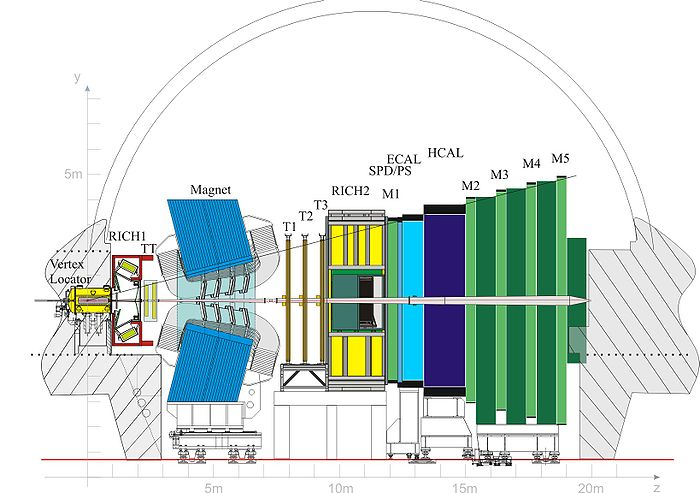
\includegraphics[scale=1]{Immagini/lhcbrivelatore}
\caption{LHCb detector, sezione longitudinale}
\label{fig:detector}
\end{figure}

\section{LHCb detector}
\noindent
Il rivelatore \`e uno spettrometro a singolo braccio, che copre una regione attorno alla linea dei fasci, di estensione angolare compreso tra i $10$ ed i $250$ mrad nel piano verticale e tra i $10$ ed i $300$ mrad nel piano orizzontale. La geometria del rilevatore \`e ottimale per la rivelazione di eventi con produzione di coppie di quark $b\bar{b}$ o $c\bar{c}$, prodotte prevalentemente in avanti e con piccola apertura angolare relativa.

Il rilevatore LHCb \`e costituito da un sistema tracciante per la determinazione delle posizioni dei vertici di produzione e decadimento dei mesoni $B$ e $D$,
per la misura dell'impulso delle tracce cariche, da un calorimetro per la rivelazione dei fotoni, e da un eccellente sistema di identificazione delle particelle. \`E inoltre dotato di un sofisticato sistema di trigger, per l'acquisizione degli eventi d'interesse, in condizioni di elevato fondo. 

\subsection{Sistemi traccianti}
\noindent
Il sistema tracciante consiste di un rivelatore dedicato alla localizzazione dei vertici primari (di collisione protone-protone dei fasci) e dei vertici secondari di decadimento dei mesoni $D$ e $B$, denominato VELO (VErtex LOcator), \`e inoltre costituito da altri quattro rivelatori traccianti (\emph{tracking stations}), posti a distanza dalla regione d' interazione dei fasci, utilizzati per la misura dell'impulso delle particelle.

Per ottenere le risoluzioni richieste i rivelatori sono stati realizzati impiegando \emph{strip} di Silicio. Le regioni pi\`u esterne delle stazioni traccianti collocate dopo il magnete sono state invece realizzate mediante rivelatori a \emph{straw tube}, impiegando cio\`e camere a deriva di forma cilindrica di diametro opportuno.

\subsubsection{Rivelatore di vertice (VELO)}
\noindent
Il VELO \`e il sistema di localizzazione dei vertici primari e secondari che consente di misurare la loro posizione con una risoluzione spaziale di circa $10\ \mu m$. 
 Si consideri che la lunghezza di volo dei mesoni $B$ da misurare, alle energie (\emph{boost}) di LHC, risulta essere in media dell'ordine del centimetro. 
Il VELO  \`e costituito da ventiquattro moduli di rivelazione, collocati attorno alla regione d'interazione, disposti in sequenza, perpendicolarmente alla linea definita dai fasci, in modo da coprire una regione di estensione complessiva di circa un metro. Ciascun modulo serve per misurare le coordinate radiale ed angolare dei segnali prodotti dalle particelle cariche che attraversano il rilevatore (\emph{hit}). A partire dalla misura delle \emph{hit} in prossimit\`a della regione d'interazione dei fasci, \`e possibile ricostruire con grande precisione la geometria delle traiettorie delle particelle cariche e localizzare con precisione i vertici primari e secondari. 
\begin{figure}[h]
\centering
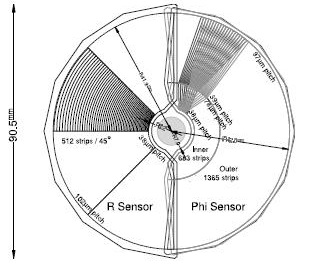
\includegraphics[scale=1]{Immagini/velo1}
\caption{Schema di uno dei ventiquattro moduli che costituiscono il rivelatore di vertice VELO di LHCb. La figura illustra la geometria dei sensori in silicio impiegati per la misura delle coordinate radiale ed angolare delle \emph{hit}.}
\label{fig:velo2}
\end{figure}
%
\subsubsection{Camere traccianti (per la misura dell'impulso).}
\noindent
Il sistema di tracciamento impiegato per la misura dell'impulso delle particelle \`e costituito dal \emph{Trigger Tracker}, posto a monte del magnete, e da tre stazioni \emph{Tracking Stations}, indicate con le sigle $T1$, $T2$ e $T3$, poste a valle di esso, come indicato in Figura \ref{fig:detector}. Ognuno di queste stazioni traccianti \`e costituta da quattro piani di rivelazione indipendenti, impiegati per una misura ridondante e bidimensionale delle \emph{hit } prodotte dalle particelle cariche che attraversano il rivelatore. 

Il sistema tracciante copre una superficie ortogonale alla traiettoria dei fasci pari a $150 × 130$ $cm^2$, corrispondente all'intero angolo solido di accettanza del detector.
\begin{figure}
\centering
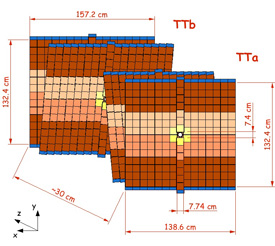
\includegraphics[scale=0.9]{Immagini/TriggerTracker}
\caption{Il sistema di tracciamento Trigger Tracker. Sono visibili i diversi settori, a diversa segmentazione, e nella parte esterna, in blu, 
i circuiti di lettura \emph{readout hybrids}.}
\label{fig:TriggerTracker}
\end{figure}
La parte pi\`u interna delle stazioni traccianti (\emph{Inner Tracker}, IT) \`e costituita da sensori al silicio, simili a quelli usati per il \emph{Trigger Tracker}, con una
differente disposizione dei sensori e segmentazione dei moduli, per le diverse esigenze di risoluzione spaziale a maggiore distanza. 
La regione esterna (\emph{Outer Tracker}, OT) \`e stata realizzata sovrapponendo quattro piani di tubi a deriva, del diametro di $5$ mm, riempiti da una miscela gassosa costituita per il $70\%$ di argon e per il $30\%$ di diossido di carbonio. La miscela permette di avere un tempo di deriva inferiore ai $50$ ns, adeguato per l'elevata frequenza di conteggio  (gli eventi si sussegguono ogni $25$ ns con occupanze medie inferiori al 10\%).
%
%
\subsection{Sistemi di identificazione delle particelle}
\noindent
Il sistema di identificazione si basa sull'uso di due rilevatori di luce Cherenkov RICH (RICH1 e RICH2), su due calorimetri ECAL ed HCAL e sul rivelatore di muoni.
\subsubsection{RICH}
\noindent
\begin{figure}
\centering
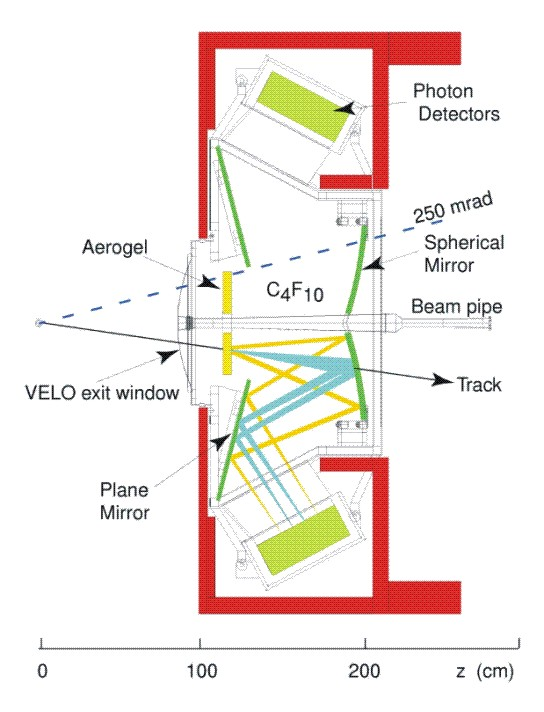
\includegraphics[scale=1.5]{Immagini/rich}
\caption{Rivelatore RICH1}
\label{fig:rich}
\end{figure}
Il riconoscimento delle particelle mediante i RICH si basa sulla misura dell'angolo Cherenkov, noto il valore dell'impulso della traccia corrispondente.

I due rivelatori RICH di LHCb (in Figura \ref{fig:rich} \`e mostrato soltanto uno di essi) sono essenziali per il riconoscimento dei decadimenti dei mesoni $D$ e $B$ in stati finali adronici. Essi permettono di distinguere le tracce dovute a pioni, kaoni e protoni che attraversano il rilevatore, in un intervallo d'impulso compreso tra $10$ ed $100$ GeV/c.

Il rivelatore RICH1 \`e posto in prossimit\`a della regione di interazione e copre per intero l'accettanza geometrica di LHCb. \`E dedicato alla rivelazione delle tracce con impulso fra $10\div60$ GeV/c. 
RICH2 \`e posto a distanza maggiore dalla regione di interazione, oltre l'ultima delle \emph{Tracking Stations}, in modo da intercettare le particelle  nell'intervallo d'impulso maggiore,  compreso tra $20$ e $100$ GeV/c. Copre una regione di angolo solido poco estesa, prossima alla linea dei fasci.

Il rilevatore RICH1 impiega due diversi mezzi radiatori: per identificare le particelle con impulso minore \`e utilizzato aerogel, un composto colloidale del quarzo, il cui indice di rifrazione \`e compreso tra $1,01$ e $1,10$; per identificare le particelle di impulso maggiore \`e utilizzato fluorobutano ($C_4F_{10}$) con indice di rifrazione $1,0014$.
Nel RICH2 \`e utilizzato tetrafluorometano ($CF_4$), con indice di rifrazione pari a $1.00048$, per rivelare le particelle della parte superiore dello spettro. La figura di merito \`e mostrata in Figura \ref{fig:rich2}
\begin{figure}
\centering
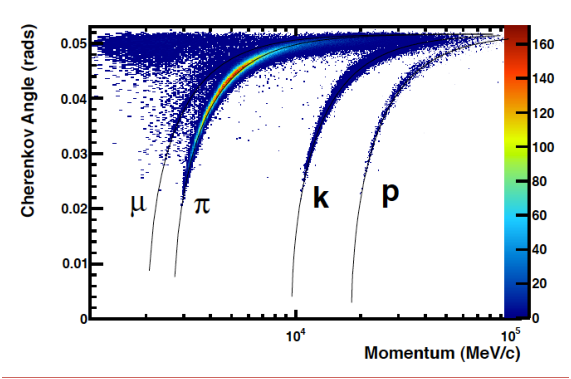
\includegraphics[scale=1.2]{Immagini/PastedGraphic-2}
\caption{Angolo di Cherenkov in funzione del mezzo radiatore e dell'impulso della particella che lo attraversa}
\label{fig:rich2}
\end{figure}

\subsubsection{Calorimetri}
\noindent
Il calorimetro adronico HCAL non \`e utilizzato \emph{offline} per l'analisi, \`e utilizzato solo in fase di trigger, per individuare eventi con adroni di elevato impulso trasversale.  
Il calorimetro elettromagnetico ECAL (con l'aggiunta di rivelatori ausiliari SPD, PS) \`e impiegato anche offline per la identificazione di fotoni, elettroni e pioni neutri.
SPD (\emph{Scintillator Pad Detector}) e PS (\emph{Preshower Detector}) forniscono segnali ausiliari ad ECAL per la discriminazione carico/neutro e la reiezione dei segnali adronici.
\begin{figure}[b]
\centering
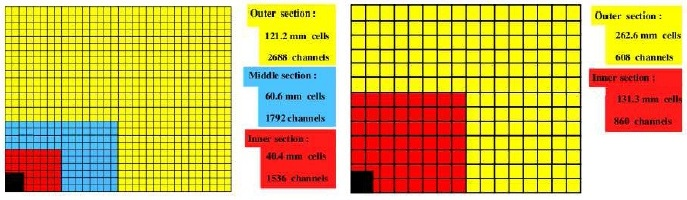
\includegraphics[scale=0.65]{Immagini/ECAL}
\caption{Schema dei calorimetri impiegati in LHCb. A destra ECAL, PS e SPD, a sinistra HCAL}
\label{fig:ECAL}
\end{figure}
ECAL \`e un calorimetro a campionamento, formato da piani assorbitori in piombo intervallati a piani sensibili di scintillatori. Analogamente HCAL \`e un calorimetro a campionamento, costituito per\`o da lastre di ferro, intervallate a scintillatori plastici. I segnali di scintillazione sono letti in entrambe i casi mediante fibre ottiche che convogliano i segnali a fotomoltiplicatori.

I calorimetri permettono di distinguere $e^\pm$ da $\pi^\pm$ con una efficienza del $90\%$ e un livello di contaminazione inferiore all'$1\%$.
La risoluzione in energia del calorimetro elettromagnetico \`e dell'ordine di qualche percento nel \emph{range} di impulso compreso tra $10$ e $100$ $GeV/c$.

\subsubsection{Rilevatore di muoni}
\begin{figure}
\centering
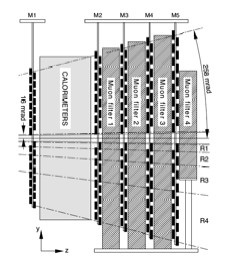
\includegraphics[scale=1]{Immagini/muon}
\caption{Rilevatore di muoni. Sono visibili le cinque camere impiegate per la rilevazione, indicate con le sigle $M_2$, $M_3$, $M_4$ ed $M_5$}
\label{fig:muon}
\end{figure}
\noindent
Poiché parte considerevole dei canali di decadimento dei mesoni $B$ e $D$ contengono muoni, la loro corretta identificazione \`e di cruciale importanza.
Il sistema di rivelazione dei muoni \`e impiega cinque stazioni di rivelazione ($M_1$, $M_2$, $M_3$, $M_4$ ed $M_5$) realizzate utilizzando camere traccianti MWPC (\emph{MultiWire Proportional Chamber}). Il sistema di rivelazione intercetta il $20\%$ dei muoni prodotti dai vari canali di decadimento del $B$ con un efficienza superiore al 95\%.
La stazione $M_1$, collocata prima dei calorimetri, deve sostenere un flusso di particelle superiore alle altre, e per questo motivo, nella regione prossima ai fasci, \`e stata  equipaggiata con rivelatori che sostengono alti rate di conteggio di tipo GEM (\emph{Gas Electron Multiplier}). Le camere $M_2$, $M_3$, $M_4$ ed $M_5$, per rivelare i muoni penetranti (perch\'e un muone superi tutte le stazioni traccianti deve avere un'energia superiore a $10$ $GeV$), sono pertanto intervallate a lastre di ferro spesse $80$ cm. Le camere traccianti hanno una risoluzione temporale inferiore a $25$ ns.

\section{Aquisizione dei dati}
\noindent
La frequenza di collisioni rivelate da LHCb \`e dell'ordine dei $10$ MHz, molto superiore alla frequenza di segnale, dell'ordine di qualche $kHz$.
Per questo motivo LHCb \`e stato dotato di un sistema di \emph{trigger} che consente di ridurre la frequenza di registrazione degli eventi a 5 $kHz$.

Il sistema di \emph{trigger} \`e strutturato su due livelli: il primo livello, chiamato L0, opera alla frequenza di \emph{bunch crossing} di LHC di $40$ MHz;
  il secondo livello, chiamato HLT (\emph{Hig Level Trigger}) opera in cascata alla frequenza di $1$ MHz.

Il trigger L0 selezione eventi con particelle di elevato impulso trasversale, mentre il trigger HLT  seleziona  eventi specifici per mezzo di algoritmi in esecuzione, in parallelo, su un \emph{cluster} di computer, costituito da alcune decine di migliaia di CPU.

Gli eventi raccolti sono inviati al centro di calcolo TIer-0 del CERN che oltre alla elaborazione di parte di essi, distribuisce i dati a sei centri di calcolo europei $Tier-1$. Fra 
i centri di calcolo vi \`e centro nazionale dell'INFN presso il CNAF di Bologna. I centri di calcolo sono utilizzati per l'elaborazione preliminare dei dati e successivamente per l'analisi utente. La produzione di eventi di simulazione \`e realizzata presso centri dedicati denominati Tier2.
